\documentclass[letterpaper,11pt]{extarticle}
 
 
\usepackage{hyperref}       % hyperlinks
\usepackage{url}            % simple URL typesetting
\usepackage{booktabs}       % professional-quality tables
\usepackage{amsfonts}       % blackboard math symbols
\usepackage{amsmath}
\usepackage{mathtools}
\usepackage{nicefrac}       % compact symbols for 1/2, etc.
\usepackage{microtype}      % microtypography
\usepackage{lipsum}
\usepackage{graphicx}
\usepackage{wrapfig}
\usepackage[left=1in,right=1in,top=1.5in,bottom=1.8in]{geometry}
\usepackage{xcolor}
\usepackage{setspace} 
\usepackage{subcaption}
\usepackage{caption}
\usepackage{gensymb}
\usepackage[]{algorithm2e}
\usepackage[font=small,labelfont=bf]{caption}
\definecolor{saycolor}{HTML}{21618C}
\newcommand{\say}[1]{\textcolor{saycolor}{#1}}
\usepackage[normalem]{ulem}  % for \sout{}
\usepackage{advdate}

 
% -- math operator for argmax and argmin
\DeclareMathOperator*{\argmax}{arg\,max}
\DeclareMathOperator*{\argmin}{arg\,min}
 
 
\title{Deep Gaussian Processes: A Survey}
 
\begin{document}

\author{Kalvik~Jakkala}

\maketitle

\begin{abstract}
The abstract goes here.
\end{abstract}


\section{Introduction}
There have been numerous advances in the field of machine learning in recent years. Most of these advances can be primarily attributed to backpropagation, large datasets, and computational resource improvements. However, most of the currently popular machine learning approaches mainly, deep learning methods, are based on frequentist approaches, which entail making any prediction decisions primarily by studying the correlations among features and predictions in a dataset. The problem with such an approach is that it is easy to overfit to the available dataset and risk learning unwanted biasing in the dataset. 

Furthermore, current approaches make it difficult and unintuitive to introduce any prior domain knowledge into a model. Although it is not always the case, several real-world problems might domain experts whose knowledge might help develop good models. Most deep learning approaches do not accommodate such incorporations and require application-specific methods to be developed to address such an issue.

Prediction uncertainty is an important metric that needs to be estimated by reliable models. Most data sources contain non-negligible quantities of noise that might hinder the performance of a prediction model. Moreover, it is also not uncommon to have test time data samples that do not closely resemble the training dataset. In such cases, it is essential to know how certain a model is about its prediction. If the model were to be used in a mission-critical task and not take the model's prediction uncertainty, it could lead to catastrophic results. 

Another major drawback of conventional deep learning approaches is model comparison. Deep learning approaches are parametric and require explicit definitions for the model architecture. Moreover, these model architectures need to be developed for each application separately. Often multiple model architectures need to be compared against each other to determine which is the best. However, it is nontrivial to factor in model size in terms of its parameters and accuracy for comparison. 

The limitations mentioned above are addressed by Bayesian approaches with varying degrees of ease and efficiency. Domain knowledge can be incorporated with a prior distribution, uncertainty of predictions can be estimated with prediction variance, and the model can be appropriately compared with the Bayes factor.

Apart from the advantages mentioned above of Bayesian approaches, another interesting feature of Bayesian methods is that they facilitate causal modeling \cite{PearlM18} of any system or process being modeled. Indeed, most classification or regression problems entail a chain of sub-decisions, each of which would to the end prediction. However, conventional deep learning approaches are not particularly amenable to specifying such causal models. The Bayesian framework, along with do-calculus, can be used to specify such structures in models. 

The advantages of Bayesian approaches raise the question of why they do not have a more widespread adaptation. Indeed, Bayesian approaches often incur heavy computational expense or outright intractabilities that make them infeasible for several problems. Nonetheless, these methods are steeped with history and have been used to solve numerous problems with substantial ramifications \cite{Mcgrayne11}. Time and time again, the Bayesian framework has proved itself to be worthy. 

This paper considers one particular type of Bayesian approach, i.e., Gaussian processes \cite{RasmussenW06}. The method has its roots in Stochastic processes—a field of study dedicated to modeling random processes with Probability theory \cite{Klebaner12,Rosenthal06}. Most problems of interest are usually not deterministic processes, or even if they are, one might not have access to all the information needed to model it as such. Stochastic processes mathematically accommodate such uncertainties, and Gaussian processes are one particular variant of Stochastic processes. 

We start our exposition by detailing Gaussian processes, their advantages, and disadvantages. Furthermore, we describe some of the prominent variants of Gaussian Processes that were crucial for building deep Gaussian processes. Finally, we explain some of the critical deep Gaussian process approaches. 

\section{Preliminary}

A collection of random variables is called a Gaussian Process(GPs) if the joint distribution of any finite number of its members is a Gaussian. Gaussian processes can be thought of as a reinterpretation or a generalization of Gaussian distributions. Gaussian processes are essentially Gaussian distributions with  $\infty$ dimensions. Each dimension of the distribution corresponds to an input data sample, and the distribution mean represents each data input's associated label. 

Gaussian processes are fascinating because of their analytical properties. Gaussian processes being Gaussian distributions have closed-form analytical solutions to summation, conditioning, and marginalization under certain conditions, as shown below. These properties make them amenable to reasonable computation costs while retaining their Bayesian properties. For a distribution defined by the following mean and covariance, 

$$
\boldsymbol{\mu}=\left(\begin{array}{l}
\boldsymbol{\mu}_{1} \\
\boldsymbol{\mu}_{2}
\end{array}\right), \quad \boldsymbol{\Sigma}=\left(\begin{array}{ll}
\boldsymbol{\Sigma}_{11} & \boldsymbol{\Sigma}_{12} \\
\boldsymbol{\Sigma}_{21} & \boldsymbol{\Sigma}_{22}
\end{array}\right), \quad \boldsymbol{\Lambda}=\boldsymbol{\Sigma}^{-1}=\left(\begin{array}{ll}
\boldsymbol{\Lambda}_{11} & \boldsymbol{\Lambda}_{12} \\
\boldsymbol{\Lambda}_{21} & \boldsymbol{\Lambda}_{22}
\end{array}\right)
$$
the marginals are given by
$$
\begin{aligned}
p\left(\mathbf{x}_{1}\right) &=\mathcal{N}\left(\mathbf{x}_{1} \mid \boldsymbol{\mu}_{1}, \boldsymbol{\Sigma}_{11}\right) \\
p\left(\mathbf{x}_{2}\right) &=\mathcal{N}\left(\mathbf{x}_{2} \mid \boldsymbol{\mu}_{2}, \mathbf{\Sigma}_{22}\right)
\end{aligned}
$$
and the conditionals are given by
$$
\begin{aligned}
p\left(\mathbf{x}_{1} \mid \mathbf{x}_{2}\right) &=\mathcal{N}\left(\mathbf{x}_{1} \mid \boldsymbol{\mu}_{1 \mid 2}, \boldsymbol{\Sigma}_{1 \mid 2}\right) \\
\boldsymbol{\mu}_{1 \mid 2} &=\boldsymbol{\mu}_{1}+\boldsymbol{\Sigma}_{12} \boldsymbol{\Sigma}_{22}^{-1}\left(\mathbf{x}_{2}-\boldsymbol{\mu}_{2}\right) \\
&=\boldsymbol{\mu}_{1}-\boldsymbol{\Lambda}_{11}^{-1} \boldsymbol{\Lambda}_{12}\left(\mathbf{x}_{2}-\boldsymbol{\mu}_{2}\right) \\
&=\boldsymbol{\Sigma}_{1 \mid 2}\left(\boldsymbol{\Lambda}_{11} \boldsymbol{\mu}_{1}-\boldsymbol{\Lambda}_{12}\left(\mathbf{x}_{2}-\boldsymbol{\mu}_{2}\right)\right) \\
\boldsymbol{\Sigma}_{1 \mid 2} &=\boldsymbol{\Sigma}_{11}-\boldsymbol{\Sigma}_{12} \boldsymbol{\Sigma}_{22}^{-1} \boldsymbol{\Sigma}_{21}=\mathbf{\Lambda}_{11}^{-1}
\end{aligned}
$$

Moreover, as mentioned before, deep neural networks require the specification of model architectures which are usually application-specific.  However, GPs do not suffer from such issues as they are non-parametric. GPs consider the entire function space and marginalize it to obtain a prediction. Such a process allows two main advantages. The first one need not decide the complexity of the model apriori, and the second, the marginalization process incuses a natural Razor's Occum, thereby overcoming any overfitting issues. 
 
One might wonder if modeling any arbitrary process as a Gaussian would result in poor performance. However, Gaussians are omnipresent, and the Central Limit Theorem applies to them. The theorem states that any data's mean and variance follow a Gaussian distribution as the number of samples from a distribution increases; this applies to data from the distribution. 

Another interesting property of Gaussians is that the distribution has the maximum entropy given a data mean and variance \cite{Murphy12}. The first two moments, mean and variance, are usually the only metrics that we can accurately compute from data. As a result, using Gaussians to estimates distributions results in the most informative data distribution estimates. 

Finally, another important property of Gaussian processes was established by Neil in \cite{Neal96} where he showed that GPs are equivalent to a single-layered Perceptron with $\infty$ hidden units. Such perceptions are, in turn, known to be universal approximators that can approximate any function given enough data \cite{HornikSW89}. 

\section{Gaussian Processes}
We have detailed the critical advantages of Bayesian approaches and why we are interested in Gaussian processes specifically. This section further elaborates on GPs. Indeed, we give an intuition of GPs, their mathematical formulation \cite{RasmussenW06, Murphy12}, and an interpretation of the terms in its formulation.  This is followed by explaining Kernel functions and some of the limitations of GPs. 

\begin{figure}[htp]
    \centering
    \includegraphics[width=\linewidth]{figs/GP_ill.pdf}
    \caption{Illustration of a Gaussian Process.}
    \label{fig:mnist_gp}
\end{figure}

GPs, as mentioned before, are essentially Gaussian distributions interpreted as probabilistic mappings from some data input space to output label space. This mapping has a convenient interpretation in the function space. Formally, we assume a function $f$, maps an input space $x$ to the output space $y$. This mapping is characterized by a noise term $\epsilon$.
$$
\mathbf{y}=f(\mathbf{x})+\boldsymbol{\epsilon}, \boldsymbol{\epsilon} \sim \mathcal{N}\left(\mathbf{0}, \beta^{-1} \mathbf{I}\right)
$$
In a non-probabilistic approach, one would consider a parametric form for the function $f$ and use Maximum A Posteriori (MAP) to determine its parameters. GPs, on the other hand, assume a distribution over the functions. And any predictions entail marginalizing over the entire function space. The distribution over the functions is defined by vector mean term and a covariance matrix that is usually determined by the kernel function. 
$$
\begin{aligned}f|\mathbf{x} & \sim \mathcal{G} \mathcal{P}\left(\mu(\mathbf{x}), k_{f}\left(\mathbf{x}, \mathbf{x}^{\prime}\right)\right) \\
\mu(\mathbf{x}) &=\mathbb{E}[f(\mathbf{x})] \\
k_{f}\left(\mathbf{x}, \mathbf{x}^{\prime}\right) &=\mathbb{E}\left[(f(\mathbf{x})-\mu(\mathbf{x}))\left(f\left(\mathbf{x}^{\prime}\right)-\mu\left(\mathbf{x}^{\prime}\right)\right)\right]
\end{aligned}
$$
Moreover, by treating the function outputs as noisy versions of the labels, the distribution over $y$ conditioned on the input $X$ can be achieved as follows. 
$$
p(\mathbf{y} \mid \mathbf{f})=\mathcal{N}\left(\mathbf{f}, \beta^{-1} \mathbf{I}\right) \\
p(\mathbf{y} \mid X)=\int p(\mathbf{y} \mid \mathbf{f}) p(\mathbf{f} \mid X) d \mathbf{f}
$$
The above would allow for computing the probability of a dataset. We are usually interested in predicting the label for new data, which we can achieve by considering a joint distribution over the latent values from both the training dataset and testing dataset produced by the function $f$.     
$$
\left[\begin{array}{l}
\mathbf{f} \\
\mathbf{f}_{*}
\end{array}\right] \sim \mathcal{N}\left(\mathbf{0},\left[\begin{array}{ll}
K(X, X) & K\left(X, X_{*}\right) \\
K\left(X_{*}, X\right) & K\left(X_{*}, X_{*}\right)
\end{array}\right]\right)
$$
The distribution of $f_*$ can be obtained by conditioning it with $X_*$, $X$, and $y$ as follows. 
$$
p(\mathbf{f_*} \mid X_*, X, y) = \frac{1}{p({\mathbf{y}})} \int p(\mathbf{y} \mid \mathbf{f}) p(\mathbf{f}, \mathbf{f_*}) d \mathbf{f}
$$
$$
\begin{aligned}
p(\mathbf{f_*} \mid X_*, X, y) \sim \mathcal{N}(& K\left(X_{*}, X\right) K(X, X)^{-1} \mathbf{f} \\
&\left.K\left(X_{*}, X_{*}\right)-K\left(X_{*}, X\right) K(X, X)^{-1} K\left(X, X_{*}\right)\right)
\end{aligned}
$$
Note that we are not interested in the distribution of $y_*$ as it is just a noise induced version of $f$. Moreover, the mean of the conditional distribution above can be considered the model prediction as a Gaussian distribution's mode coincides with its mean.

The mean term of the predictive distribution can be interpreted as taking a weighted average of the training set labels with the weights defined by the kernel matrices, which quantify the two inputs' similarity. The variance term has two parts. The first term on the left can be assumed to be the prior variance of the testing data and, the second term can be thought of as the reduction of variance induced by the training set data. 

\subsection{Kernel Function}
As we briefly mentioned before, the kernel function is a function that measures the similarity of input data.  Unlike a conventional Gaussian distribution, since a GP has $\infty$ dimensions, explicitly defining a kernel matrix would be infeasible in most cases. We resort to using kernel functions which allow for a more compact approach to specifying the kernel matrix. 

Kernel functions must produce a positive semi-definite (PSD). Any function which meets the criteria can be used as a kernel function. Kernel functions can be interpreted as dot products between data points in a high dimensional manifold without explicitly mapping the data points to such a manifold, which allows us to define meaningful similarity metrics relevant for a given task.  

Numerous kernel functions are used in literature, each with its own set of properties that make it useful for different tasks. Enumerating and explaining all such functions is out of this paper's scope, and the readers are referred to \cite{RasmussenW06} for a detailed overview. However, two main functions are often used in literature, particularly the Squared Exponential Kernel and the Automatic Relevance Detection Kernel functions that we detail below. 

The Squared Exponential Kernel, also known as the Radial Basis Function and Gaussian Kernel, has an exponential form. It has two parameters, the length scale $\ell$, which determines how far a pair of data points need to be correlated, and the variance scale $\sigma$, which quantifies the variance induced from data points. The function is parameter efficient as it has only two parameters and its form allows for analytical computations of integrals involving the function. 
$$
k_{f(\mathrm{EQ})}\left(\mathbf{x}_{i,:}, \mathbf{x}_{k,:}\right)=\sigma^{2} \exp \left(-\frac{1}{2 \ell^{2}} \sum_{j=1}^{q}\left(x_{i, j}-x_{k, j}\right)^{2}\right)
$$
Another important kernel function is the Automatic Relevance Detection Kernel. It has a similar form to the Gaussian kernel, but it has weight parameters for each dimension of the input space. We can use the weight parameters to change the importance of any feature in the inputs, and if needed, they can even be used to disable irrelevant features altogether. 

$$
k_{f(\mathrm{ARD})}\left(\mathbf{x}_{i,:}, \mathbf{x}_{k,:}\right)=\sigma_{\mathrm{ARD}}^{2} \exp \left(-\frac{1}{2} \sum_{j=1}^{q} w_{j}\left(x_{i, j}-x_{k, j}\right)^{2}\right)
$$
The weight parameter in the kernel functions can be manually defined, but, often, such an approach is rather infeasible. In practice, such parameters are usually determined from any available training data itself, which allows us to obtain kernel functions that are most suited to describe a dataset. Indeed, there are two primary approaches to determine the function parameters, MAP and the Bayesian approach. 

The Maximum A Posteriori (MAP) approach considers the log probability of the dataset $\log p(\mathbf{y} \mid X)$. The optimal parameters are computed by taking the derivative of the dataset's log probability with respect to the kernel parameters. Depending on the dataset size, the parameters can be calculated analytically but, in some cases, one needs to resort to approaches like gradient descent to determine the parameters. 

$$
\log p(\mathbf{f} \mid X)=-\frac{1}{2} \mathbf{f}^{\top} K^{-1} \mathbf{f}-\frac{1}{2} \log |K|-\frac{n}{2} \log 2 \pi \\
$$
$$
\log p(\mathbf{y} \mid X)=-\frac{1}{2} \mathbf{y}^{\top}\left(K+\sigma_{n}^{2} I\right)^{-1} \mathbf{y}-\frac{1}{2} \log \left|K+\sigma_{n}^{2} I\right|-\frac{n}{2} \log 2 \pi
$$
One limitation of using MAP to determine the kernel parameters is that it could lead to overfitting. The problem's severity varies depending on the dataset size, the GP's variant, and the kernel function being used. We can mitigate the problem by using a Bayesian approach. In such an approach, one defines a distribution over the kernel parameters and computes the posterior parameter distribution conditioned on the training dataset. 

Although the Bayesian approach is ideal, it is usually intractable to analytical computations of the parameter distributions. So, one has to resort to sampling approaches such as Hamiltonian Monte Carlo methods to determine the parameter distribution. However, such methods have their limitations and introduce additional computational costs that might be infeasible. 

\subsection{Limitations}

Although GPs have several advantages, they also have a few key limitations which hinder their use in most machine learning problems. Particularly, there are three key problems:

\begin{enumerate}
\item Computation cost
\item Storage cost
\item Depth
\end{enumerate}

\begin{figure}[htp]
    \centering
    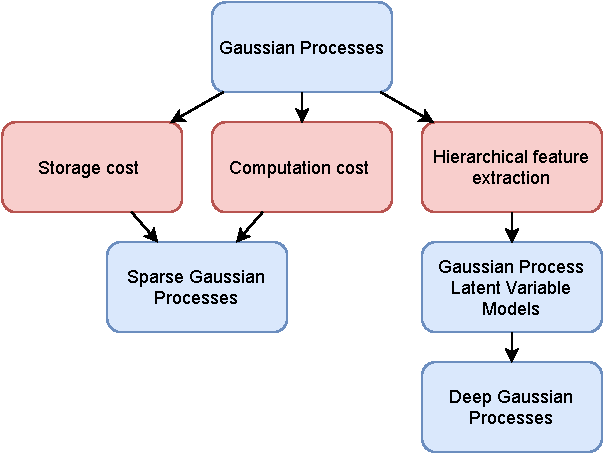
\includegraphics[width=0.6\linewidth]{figs/GP.pdf}
    \caption{Overview of Gaussian Processes and their variants.}
    \label{fig:overview}
\end{figure}

The computational cost of GPs can be rather substantial; this is because, to get the predictive distribution of a GP, one needs to invert the kernel matrix. The kernel matrix's size is $n \times n$ where $n$ is the number of data points in the training dataset. Inverting such a matrix takes $O(n^3)$ computation time. Although, this is only for the training phase. It takes $O(n)$ and $O(n^2)$ time to determine the predictive distribution's mean and variance of a new data point.

Similar to the computational cost, since GPs require the entire training dataset's storage, making the storage cost $O(n^2)$. Depending on the size of the dataset could be completely infeasible. Moreover, if the GP were to be used in an environment where the training dataset size keeps increasing, the computation and storage costs could overwhelm the entire process, rendering the benefits of GP far too expensive. As such, GPs are usually only feasible for datasets with about $1000-3000$ data points.

Another major drawback of GPs is using them on structured data wherein one needs to consider hierarchical feature extraction to determine the similarity of a pair of data points properly. Such an issue often arises in data such as images but, it is also prevalent in simpler vector datasets. Conventional kernel functions are ill-equipped to handle such correlations, and one needs to resort to deep feature extraction like the ones used in Deep learning models. However, such feature extraction still needs to be confined to a Bayesian framework to retain a GP's advantages.

Sparse Gaussian Processes address the computational and storage costs. And the depth issue is addressed by Deep Gaussian Processes. We explain some of the prominent methods for Sparse and Deep GPs that have been developed over the last two decades. 

\section{Sparse Gaussian Processes}

Given the computational and storage requirements that hinder the widespread use of GPs, a substantial number of papers have tried to address the problem and are usually referred to as Sparse Gaussian Processes (SGPs). The terminology stems from the way most of these approaches address the issue. Because the primary problem is the inversion of a covariance matrix, most methods try to introduce sparsity and reduce the matrix size that needs to be inverted while retaining the performance achieved while using the full size matrix. 

A complete overview of all SGPs is 
outside this survey's scope; the readers are referred to \cite{LiuOSC20} for a thorough summary. This section focuses only on some of the well-known methods that are crucial for developing some of the Deep Gaussian Process methods that will be detailed in the upcoming section. 

The Nyström approximation of \cite{WilliamsS01} is a well know approach to reducing the covariance of the training set $K_{x, x}$. The Nyström approximation allows one to generate a low rank approximation of any kernel matrix. The approach is applied to GPs by selecting $m$ data points with $m<<n$  from the training set and computing the approximation to the kernel matrix $\tilde{K}$ which has to size $m \times m$ as follows

$$\tilde{K} = K_{n,m} K_{m,m}^{-1}  K_{m,n}$$

The approximation assumes that the data comes from a low rank manifold, which would be the case if the data dimension $d<n$. In such a case, the low rank approximation would be exact and result in no information loss.  However, the selected data points also influence the approximation. It is possible to have data points that result in a poor approximation even if the data is from a low dimensional manifold. Moreover, the method does not return a good approximation when the true kernel matrix lies in a high dimensional manifold.  

\begin{wrapfigure}{r}{0.5\textwidth}
  \begin{center}
    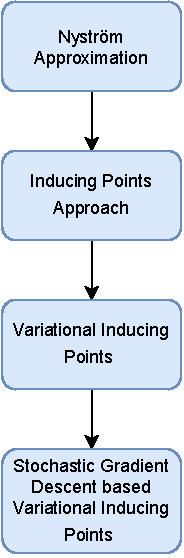
\includegraphics[width=0.2\textwidth]{figs/SGP.pdf}
  \end{center}
    \caption{Overview of Sparse Gaussian Processes.}
    \label{fig:sgp}
\end{wrapfigure}

In practice, most datasets have more data points than the number of features; thus, the method is applicable in most cases. But, since selecting the data points is crucial to the approximation's performance, one needs to take great care in doing so. Williams and Seeger used a random subset in their approach  \cite{WilliamsS01}. Although the methods work, the unsophisticated data selection process limited th method's applicability. 

Snelson and Ghahramani \cite{SnelsonEZ06} addressed selecting the training data subset for approximating the true kernel by treating the approximation subset as model parameters termed pseudo dataset. The pseudo data is assumed to be synthetic and does not necessarily correspond to any data point available in the training dataset. The pseudo points were computed using maximum likelihood. 

However, to compute the pseudo points using maximum likelihood, one needs to parameterize the GP with pseudo points appropriately. Snelson and Ghahramani \cite{SnelsonEZ06} considered a joint distribution over latent representations of data from both the training set and the pseudo points. The authors then marginalized the pseudo points to obtain the predictive distribution. 

$$
\begin{array}{l}
p\left(\mathbf{f}_{*}, \mathbf{f}\right)=\int p\left(\mathbf{f}_{*}, \mathbf{f}, \mathbf{m}\right) \mathrm{d} \mathbf{m}=\int p\left(\mathbf{f}_{*}, \mathbf{f} \mid \mathbf{m}\right) p(\mathbf{m}) \mathrm{d} \mathbf{m} \\
p(\mathbf{m})=\mathcal{N}\left(\mathbf{0}, K_{\mathbf{m}, \mathbf{m}}\right)
\end{array}
$$

Although using maximum likelihood to determine the pseudo points' distribution works in practice, using maximum likelihood runs the risk of overfitting to the training dataset. Using a Bayesian approach to compute the pseudo points posterior distribution upon conditioning with the training set would be ideal. Unfortunately, such an approach is infeasible as it becomes intractable to analytical solutions of the pseudo points.
$$
\begin{array}{c}
p(\mathbf{y} \mid \mathbf{X}, \overline{\mathbf{X}}, \overline{\mathbf{f}})=\mathcal{N}\left(\mathbf{y} \mid \mathbf{K}_{N M} \mathbf{K}_{M}^{-1} \overline{\mathbf{f}}, \mathbf{\Lambda}+\sigma^{2} \mathbf{I}\right) \\
\mathbf{\Lambda}=\operatorname{diag}(\boldsymbol{\lambda}), \lambda_{n}=K_{n n}-\mathbf{k}_{n}^{\top} \mathbf{K}_{M}^{-1} \mathbf{k}_{n}, \text { and }\left[\mathbf{K}_{N M}\right]_{n m}=K\left(\mathbf{x}_{n}, \overline{\mathbf{x}}_{m}\right)
\end{array}
$$

Moreover, the approach works by assuming that the joint distribution $p\left(\mathbf{f}_{*}, \mathbf{f}\right)$ can be partitioned as follows

$$
p\left(\mathbf{f}_{*}, \mathbf{f}\right) =\int p\left(\mathbf{f}_{*}, \mid \mathbf{m}\right)p\left(\mathbf{f} \mid \mathbf{m}\right) p(\mathbf{m}) \mathrm{d} \mathbf{m} \\
$$

The assumption limits the information a GP obtains from the training set to be induced only through the pseudo set. Hence, the pseudo points are also referred to as inducing inputs. The factorization assumption limits the capacity of the model and affects the accuracy of the model. Notably, the prior distribution that is assumed for the pseudo set substantially influences the results. 

Snelson and Ghahramani \cite{SnelsonEZ06} treated the pseudo points as hyperparameters and introduced a prior over them, resulting in an inaccurate posterior compared to a vanilla GP. Titsias \cite{Titsias09} addressed the outfitting and inexact posterior issue by considering a variational approach. The approach introduces a lower bound that can be optimized to determine the inducing inputs and the kernel hyperparameters. 

$$
F_{V}\left(X_{m}\right)=\log \left[N\left(\mathbf{y} \mid \mathbf{0}, \sigma^{2} I+Q_{n n}\right)\right]-\frac{1}{2 \sigma^{2}} \operatorname{Tr}(\widetilde{K})
$$

The marginal in \cite{Titsias09} didn't have the factorization required to apply stochastic gradient descent. Hensman et al. \cite{HensmanFL13} improved on the work of Titsias \cite{Titsias09} by developing a tighter bound that could be optimized with stochastic gradient descent. Unlike Titsias's approach, the method in \cite{HensmanFL13} did not require the entire dataset at once to compute the variational parameters. It used the following bound that could be optimized with stochastic gradient descent. 
$$
\begin{aligned}
\mathcal{L}_{3}=\sum_{i=1}^{n}\{& \log \mathcal{N}\left(y_{i} \mid \mathbf{k}_{i}^{\top} \mathbf{K}_{m m}^{-1} \mathbf{m}, \beta^{-1}\right) \\
&\left.-\frac{1}{2} \beta \widetilde{k}_{i, i}-\frac{1}{2} \operatorname{tr}\left(\mathbf{S} \mathbf{\Lambda}_{i}\right)\right\} \\
&-\mathrm{KL}(q(\mathbf{u}) \| p(\mathbf{u}))
\end{aligned}
$$

\section{Gaussian Process Latent Variable Model}
The methods discussed so far primarily addressed the computation and storage cost issues. This section introduces a variant of GPs that can be trained in an unsupervised manner. We can train Gaussian Process Latent Variable Models (GPLVMs) either in an entirely unsupervised way or in a semi-supervised manner. Although it seems irrelevant, the approach plays a significant role in some of the Deep Gaussian Processes that we will cover in the next section. 

Lawrence \cite{Lawrence04,Lawrence05} developed GPLVM. He showed that if the function space of a GP is constrained to linear function space, the GP is equivalent to Principal Component Analysis (PCA). Moreover, if the function space is relaxed to a kernel function, it can be interpreted as probabilistic non-linear PCA. The approach worked by assuming a standard Gaussian prior over the input dataset and maximizing the log probability of the dataset $p( \mathbf{Y}| \mathbf{X}, \beta)$ with respect to the input data likelihood $\mathbf{X}$. 

The unknown input data set $\mathbf{X}$ could not be computed analytically with the approach because of non-linearities introduced by the kernel function. However, Lawrence \cite{Lawrence04, Lawrence05} showed that the dataset could be computed using the Expectation-Maximization algorithm. But, the approach would return only the mode of the data distribution as a consequence. ,
$$
\frac{\partial L}{\partial \mathbf{K}}=\mathbf{K}^{-1} \mathbf{Y} \mathbf{Y}^{\mathrm{T}} \mathbf{K}^{-1}-D \mathbf{K}^{-1}
$$
Moreover, GPLVMs were shown to be useful for reconstructing inputs from a partially observed dataset. Such a scenario often occurs in image reconstruction or denoising tasks.

Although GPLVMs were very useful for unsupervised tasks, the original method assumed access to the whole kernel matrix, which entailed storing the entire training dataset and inverting a $n \times n$ kernel matrix. Lawrence \cite{Lawrence07} addressed this issue by showing that most sparse Gaussian process approaches can be turned into a GPLVM. However, the approach still gave a MAP estimate and risked overfitting to the training dataset. 

Titsias and Lawrence \cite{TitsiasL10} addressed the overfitting issue by proposing a Bayesian approach. Instead of finding a MAP solution to the data, Titsias and Lawrence proposed a variational approach. However, using the vanilla variational approach to finding the data likelihood introduces intractabilities. Titsias and Lawrence addressed the problem by incorporating Titsias's variational approach to SGPs \cite{Titsias09}. The introduction of pseudo points from the variational approach \cite{Titsias09} canceled out the intractable terms and returns the appropriate result upon optimizing the presented bound. 
$$
\begin{aligned}
\log p\left(\mathbf{y}_{d} \mid X\right) & \geq \int \phi\left(\mathbf{u}_{d}\right) \log \frac{p\left(\mathbf{u}_{d}\right) \mathcal{N}\left(\mathbf{y}_{d} \mid \boldsymbol{\alpha}_{d}, \beta^{-1} I_{N}\right)}{\phi\left(\mathbf{u}_{d}\right)} d \mathbf{u}_{d} \\
&-\frac{\beta}{2} \operatorname{Tr}\left(K_{N N}-K_{N M} K_{M M}^{-1} K_{M N}\right)
\end{aligned}
$$
GPLVMs have been applied to numerous applications and their variants that we did not cover here. The readers are referred to \cite{LiC16} for an in-depth survey of GPLVMs. 

\section{Deep Gaussian Processes}
Although SGPs addressed the computation cost issue, GPs remain inapplicable to a lot of applications. The reason being the kernel function. The most commonly used kernel functions have relatively simple similarity metrics. However, in specific datasets, one might have to use a different similarity metric for different input space sub-regions. A similarity metric that can extract such features would have to utilize a hierarchical structure for feature extraction. 

One strategy to the problem would be to stack GPs similar to how perceptrons are stacked an MLP. But, stacking GP such that the output of one layer becomes the following layer's input makes them highly non-linear and intractable to analytical solutions. Moreover, a stacked GP would not even correspond to a GP anymore as the posterior distribution can take on any arbitrary distribution. Such methods are usually referred to as Deep Gaussian Processes (DGPs). Several authors have tried to model and fit such models; this section explains such methods' development. 

One of the earliest DGP approaches is that of Lawrence and Moore \cite{LawrenceM07}. They considered a GPLVM model, but a GP was assumed for the input space prior to making it a two layered DGP. The DGP resulted in the following likelihood function, which cannot be marginalized. 

$$
p\left(\mathbf{Y}\mid\mathbf{t}\right) =\int p\left(\mathbf{Y}\mid\mathbf{X}\right) p\left(\mathbf{X}\mid\mathbf{t}\right)\mathrm{d} \mathbf{X} \\
$$

Lawrence and Moore the authors considered a MAP solution to the above problem. This was achieved by maximizing the following. 
$$
p\left(\mathbf{X}\mid\mathbf{Y, t}\right) =\log p\left(\mathbf{Y}\mid\mathbf{X}\right) + \log p\left(\mathbf{X}\mid\mathbf{t}\right) + \text {const} \\
$$

Using gradient based approaches, one could find the solution to the model. The authors also showed that deeper hierarchies could be modeled with such an approach. However, the model will be limited to a MAP solution which is highly susceptible to overfitting.  

Damianou et al. \cite{DamianouTL11} proposed a variational approach to the overfitting problem. They considered a 2-layered stacked GP, but the variational bound for such a model introduces intractabilities similar to a GPLVM.  Damianou et al. showed that the variational approach used for Bayesian GPLMVs in \cite{TitsiasL10} could also be utilized to formulate a variational bound for a 2-layered GP. The final bound is shown below

$$
\mathcal{F}_{v}(q, \boldsymbol{\theta})=\hat{\mathcal{F}}_{v}-\operatorname{KL}(q(X) \| p(X \mid \mathbf{t})) \\
\hat{\mathcal{F}}_{v}=\int q(X) \log p(Y \mid F) p(F \mid X) \mathrm{d} X \mathrm{~d} F
$$
Furthermore, Damianou and Lawrence \cite{DamianouL13} improved the method in \cite{DamianouTL11}  by generalizing the variational bound to a DGP with any number of layers. The bound shown below,
$$
\mathcal{F}_{v}=\mathbf{g}_{Y}+\mathbf{r}_{X}+\mathcal{H}_{q(\mathbf{X})}-\operatorname{KL}(q(\mathbf{Z}) \| p(\mathbf{Z})) \\
\begin{array}{l}
\mathbf{g}_{Y}=g\left(\mathbf{Y}, \mathbf{F}^{Y}, \mathbf{U}^{Y}, \mathbf{X}\right) \\
\quad=\left\langle\log p\left(\mathbf{Y} \mid \mathbf{F}^{Y}\right)+\log \frac{p\left(\mathbf{U}^{Y}\right)}{q\left(\mathbf{U}^{Y}\right)}\right\rangle_{p\left(\mathbf{F}^{Y} \mid \mathbf{U}^{Y}, \mathbf{X}\right) q\left(\mathbf{U}^{Y}\right) q(\mathbf{X})} \\
\mathbf{r}_{X}=r\left(\mathbf{X}, \mathbf{F}^{X}, \mathbf{U}^{X}, \mathbf{Z}\right) \\
=\left\langle\log p\left(\mathbf{X} \mid \mathbf{F}^{X}\right)+\log \frac{p\left(\mathbf{U}^{X}\right)}{q\left(\mathbf{U}^{X}\right)}\right\rangle_{p\left(\mathbf{F}^{X} \mid \mathbf{U}^{X}, \mathbf{Z}\right) q\left(\mathbf{U}^{X}\right) q(\mathbf{X}) q(\mathbf{Z})}
\end{array}
$$
can be used on a DGP with two or more layers. Again, the crux of the approach relied on the variational trick of introducing inducing points as presented in \cite{TitsiasL10}. Damianou and Lawrence ran experiments on the MNIST dataset wherein they showed a 5-layer DGP could be used for the image classification task. 

A limitation of the {DamianouL13} is that the number of variational parameters that need to be learned increases linearly with the number of data points in the training set. And it involved inverting matrices which is a computationally expensive operation, thereby limiting its scalability. Dai et al. \cite{DaiDGL15} addressed this by introducing a back-constraint. The constraint allowed them to define the latent variables' mean terms as deterministic functions of the latent variables themselves via an MLP. The approach reduced the number of variational parameters. Moreover, Dai et al. \cite{DaiDGL15} also showed that their approach could be trained in a distributed manner, allowing the model to be scaled to large datasets.

Salimbeni and Deisenroth \cite{SalimbeniD17} recently proposed an approach that addressed the layer independence issue of prior DGP approaches. The DGP in \cite{DamianouL13} didn't model the dependencies that arise between layers; it only considered the correlations within a layer. However, Salimbeni and Deisenroth argue that such an approach is equivalent to a single GP with each input to the GP coming from a GP itself. The authors also stated that they found that some layers get turned off when using the DGP in \cite{DamianouL13}. 

Salimbeni and Deisenroth \cite{SalimbeniD17} presented a new variational bound that retains the exact model posterior similar to \cite{DamianouL13} while maintaining the correlations both within and across adjacent layers. However, Salimbeni and Deisenroth showed such an approach to be infeasible for analytic computations, but the bound can still be optimized with MCMC sampling techniques. Such an approach is computationally expensive. But, it can be parallelized by exploiting the factorization of the DGP across output dimensions. Furthermore, the method also required sampling methods during inference, but its performance is substantially better than prior works.  

$$
\mathcal{L}_{D G P}=\sum_{i=1}^{N} \mathbb{E}_{q\left(\mathbf{f}_{i}^{L}\right)}\left[\log p\left(\mathbf{y}_{n} \mid \mathbf{f}_{n}^{L}\right)\right]-\sum_{l=1}^{L} \mathrm{KL}\left[q\left(\mathbf{U}^{l}\right) \| p\left(\mathbf{U}^{l} ; \mathbf{Z}^{l-1}\right)\right]
$$

We briefly mentioned that DGPs do not necessarily correspond to Gaussian processes. Still, the methods discussed so far do model the posterior distribution as a Gaussian, each with its assumptions. Havasi et al. \cite{HavasiLF18} presented a technique that departs even more from a conventional GP. The authors show that since a Gaussian is uni-modal, using it to model the posterior will result in poor results. Instead, they suggest using a multi-modal distribution that can better capture the true posterior distribution.  

However, it is not possible to formulate an analytical to a multi-modal posterior. We can use variational inference to learn a multi-modal posterior. Still, one needs to determine the exact form of the variational distribution, which is difficult as we usually don't know the posterior distribution in advance. Havasi et al. \cite{HavasiLF18} circumvent this issue by using Stochastic Gradient Hamiltonian Monte Carlo (SGMCMC) \cite{ChenFG14} method to estimate the posterior. The approach can determine the inducing points by sampling from the true posterior instead of using a variational distribution.  

Although the approach far exceeds the performance of prior DGPs and is the current state-of-the-art, it still has its limitations. Remarkably, the SGMCMC method is difficult to tune as it introduces its parameters in addition to the ones that already have to be estimated for DGP. Several variants of MCMC methods attempt to improve upon SGMCMC, but none of those approaches have been applied to DGPs. 

The DGPs we discussed so far attempted to develop variants of GPs that can model hierarchical features in data, which was done by assuming a feed forward network with each node of the network being modeled as a GP. It is the most popular method to address the problem and has resulted in approaches that can get reasonably promising results. However, there are other approaches as well which do not consider such an explicit feed forward network. Two of the most interesting methods would be Wilson et al. \cite{WilsonHSX16} and Lee et al. \cite{LeeBNSPD18}. 

Wilson et al. \cite{WilsonHSX16} proposed a method that uses deep neural networks as the kernel function, termed deep kernel. Unlike a Gaussian kernel, the deep kernel produced a vector output, and a GP was assigned to each of the vector elements. Wilson et al. further combined the GPs with an additive structure that facilitated its training with an analytical bound. 

Wilson et al. \cite{WilsonHSX16} showed that their approach was good at several tasks. However, the deep neural network needs to be separately defined for each task, and its parameters are susceptible to overfitting given its large parameter count.  

Finally, another interesting perspective on DGPs was presented by Lee et al. \cite{LeeBNSPD18}. Until now, all the discussed GPs with linear latent functions are combined in different ways to achieve an aggregate non-linear latent function space. Lee et al. developed a method that considers an entire function space that consists of non-linear functions. The approach can be regarded as a generalization of Neil \cite{Neal96} who showed the equivalence of an infinitely wide single layer neural network to a GP. Lee et al. showed the equivalence of a GP to an infinitely wide deep neural. 

Lee et al. \cite{LeeBNSPD18} showed the approach was on par with some neural networks trained with gradient descent while retaining its uncertainty estimation. Furthermore, the uncertainty estimates were proportional to the model accuracy. But, the approach has a polynomial increasing kernel matrix making it infeasible for some problems. 
 
\section{Conclusion}
Gaussian Processes in it themselves are fascinating. Their non-parametric form, analytical properties, and ability to model uncertainty are coveted in machine learning. However, they are plagued with limitations, particularly their significant computation and storage cost. Also, conventional kernel functions restrict the family of functions that a GP could model. 

Sparse Gaussian Processes attempt to address the storage and computation cost. One dominant approach to SGPs is to use the Nyström approximation. The approach entails variational methods to model the distribution of pseudo points for a fully Bayesian treatment. There has not been any substantial work that addresses the problem mentioned above with MCMC approaches, and it remains an unexplored avenue.

Furthermore, GPLVM was a step towards DGP. However, hierarchical feature representation was not the intended use case. It was proposed as an approach for probabilistic PCA and unsupervised learning. The Bayesian GPLVM on improved upon the original method by introducing a purely Bayesian training approach. BGPLVMs facilitated the propagation of latent space uncertainty to the posterior. 

Most of the DGP approaches considered SGPs and GPLVMs to address the issue of hierarchical feature representation. The primary trend in DGPs is to stack GPs in a feedforward manner and train them with approaches used to train SGPs and GPLVMs. However, such an approach has its limitations. The optimization bounds that were developed were not always tight, and some methods were limited to analytical solutions, which imposed scalability limitations on such techniques. 

Additionally, the methods that are can be scaled to large datasets incurred substantial computational costs and required careful tuning of hyperparameters to train the model. But, there aren't any formalized rules for defining such hyperparameters that could guarantee good model convergence. The tuning issue is particularly a problem when using MCMC approaches. 

Moreover, stacking GPs makes the model parametric as it requires a predefined model depth and layer width. Lee et al. \cite{LeeBNSPD18} considered these issues and attempted to solve them by modeling the latent function space as the space of deep neural networks. But, the approach is not feasible for real world applications as of yet and requires more work to be done to get there. 

Finally, one assumption that has been prevalent in most of the methods mentioned in this paper is the factored output dimensions.  The assumption dictates that each output dimension is independent of the other dimensions. The assumption allowed for factorizations that made specific models tractable, but it might not be the case in some datasets, and it would be in an interesting line of research. 

In conclusion, GPs are an excellent approach to model datasets. The method has come a long way from its infancy, but there are still open problems that need to be addressed for it to be elevated to the prominence that it deserves. 

\bibliographystyle{IEEEtran}
\bibliography{references}
\end{document}